\documentclass[1p]{elsarticle_modified}
%\bibliographystyle{elsarticle-num}

%\usepackage[colorlinks]{hyperref}
%\usepackage{abbrmath_seonhwa} %\Abb, \Ascr, \Acal ,\Abf, \Afrak
\usepackage{amsfonts}
\usepackage{amssymb}
\usepackage{amsmath}
\usepackage{amsthm}
\usepackage{scalefnt}
\usepackage{amsbsy}
\usepackage{kotex}
\usepackage{caption}
\usepackage{subfig}
\usepackage{color}
\usepackage{graphicx}
\usepackage{xcolor} %% white, black, red, green, blue, cyan, magenta, yellow
\usepackage{float}
\usepackage{setspace}
\usepackage{hyperref}

\usepackage{tikz}
\usetikzlibrary{arrows}

\usepackage{multirow}
\usepackage{array} % fixed length table
\usepackage{hhline}

%%%%%%%%%%%%%%%%%%%%%
\makeatletter
\renewcommand*\env@matrix[1][\arraystretch]{%
	\edef\arraystretch{#1}%
	\hskip -\arraycolsep
	\let\@ifnextchar\new@ifnextchar
	\array{*\c@MaxMatrixCols c}}
\makeatother %https://tex.stackexchange.com/questions/14071/how-can-i-increase-the-line-spacing-in-a-matrix
%%%%%%%%%%%%%%%

\usepackage[normalem]{ulem}

\newcommand{\msout}[1]{\ifmmode\text{\sout{\ensuremath{#1}}}\else\sout{#1}\fi}
%SOURCE: \msout is \stkout macro in https://tex.stackexchange.com/questions/20609/strikeout-in-math-mode

\newcommand{\cancel}[1]{
	\ifmmode
	{\color{red}\msout{#1}}
	\else
	{\color{red}\sout{#1}}
	\fi
}

\newcommand{\add}[1]{
	{\color{blue}\uwave{#1}}
}

\newcommand{\replace}[2]{
	\ifmmode
	{\color{red}\msout{#1}}{\color{blue}\uwave{#2}}
	\else
	{\color{red}\sout{#1}}{\color{blue}\uwave{#2}}
	\fi
}

\newcommand{\Sol}{\mathcal{S}} %segment
\newcommand{\D}{D} %diagram
\newcommand{\A}{\mathcal{A}} %arc


%%%%%%%%%%%%%%%%%%%%%%%%%%%%%5 test

\def\sl{\operatorname{\textup{SL}}(2,\Cbb)}
\def\psl{\operatorname{\textup{PSL}}(2,\Cbb)}
\def\quan{\mkern 1mu \triangleright \mkern 1mu}

\theoremstyle{definition}
\newtheorem{thm}{Theorem}[section]
\newtheorem{prop}[thm]{Proposition}
\newtheorem{lem}[thm]{Lemma}
\newtheorem{ques}[thm]{Question}
\newtheorem{cor}[thm]{Corollary}
\newtheorem{defn}[thm]{Definition}
\newtheorem{exam}[thm]{Example}
\newtheorem{rmk}[thm]{Remark}
\newtheorem{alg}[thm]{Algorithm}

\newcommand{\I}{\sqrt{-1}}
\begin{document}

%\begin{frontmatter}
%
%\title{Boundary parabolic representations of knots up to 8 crossings}
%
%%% Group authors per affiliation:
%\author{Yunhi Cho} 
%\address{Department of Mathematics, University of Seoul, Seoul, Korea}
%\ead{yhcho@uos.ac.kr}
%
%
%\author{Seonhwa Kim} %\fnref{s_kim}}
%\address{Center for Geometry and Physics, Institute for Basic Science, Pohang, 37673, Korea}
%\ead{ryeona17@ibs.re.kr}
%
%\author{Hyuk Kim}
%\address{Department of Mathematical Sciences, Seoul National University, Seoul 08826, Korea}
%\ead{hyukkim@snu.ac.kr}
%
%\author{Seokbeom Yoon}
%\address{Department of Mathematical Sciences, Seoul National University, Seoul, 08826,  Korea}
%\ead{sbyoon15@snu.ac.kr}
%
%\begin{abstract}
%We find all boundary parabolic representation of knots up to 8 crossings.
%
%\end{abstract}
%\begin{keyword}
%    \MSC[2010] 57M25 
%\end{keyword}
%
%\end{frontmatter}

%\linenumbers
%\tableofcontents
%
\newcommand\colored[1]{\textcolor{white}{\rule[-0.35ex]{0.8em}{1.4ex}}\kern-0.8em\color{red} #1}%
%\newcommand\colored[1]{\textcolor{white}{ #1}\kern-2.17ex	\textcolor{white}{ #1}\kern-1.81ex	\textcolor{white}{ #1}\kern-2.15ex\color{red}#1	}

{\Large $\underline{11a_{183}~(K11a_{183})}$}

\setlength{\tabcolsep}{10pt}
\renewcommand{\arraystretch}{1.6}
\vspace{1cm}\begin{tabular}{m{100pt}>{\centering\arraybackslash}m{274pt}}
\multirow{5}{120pt}{
	\centering
	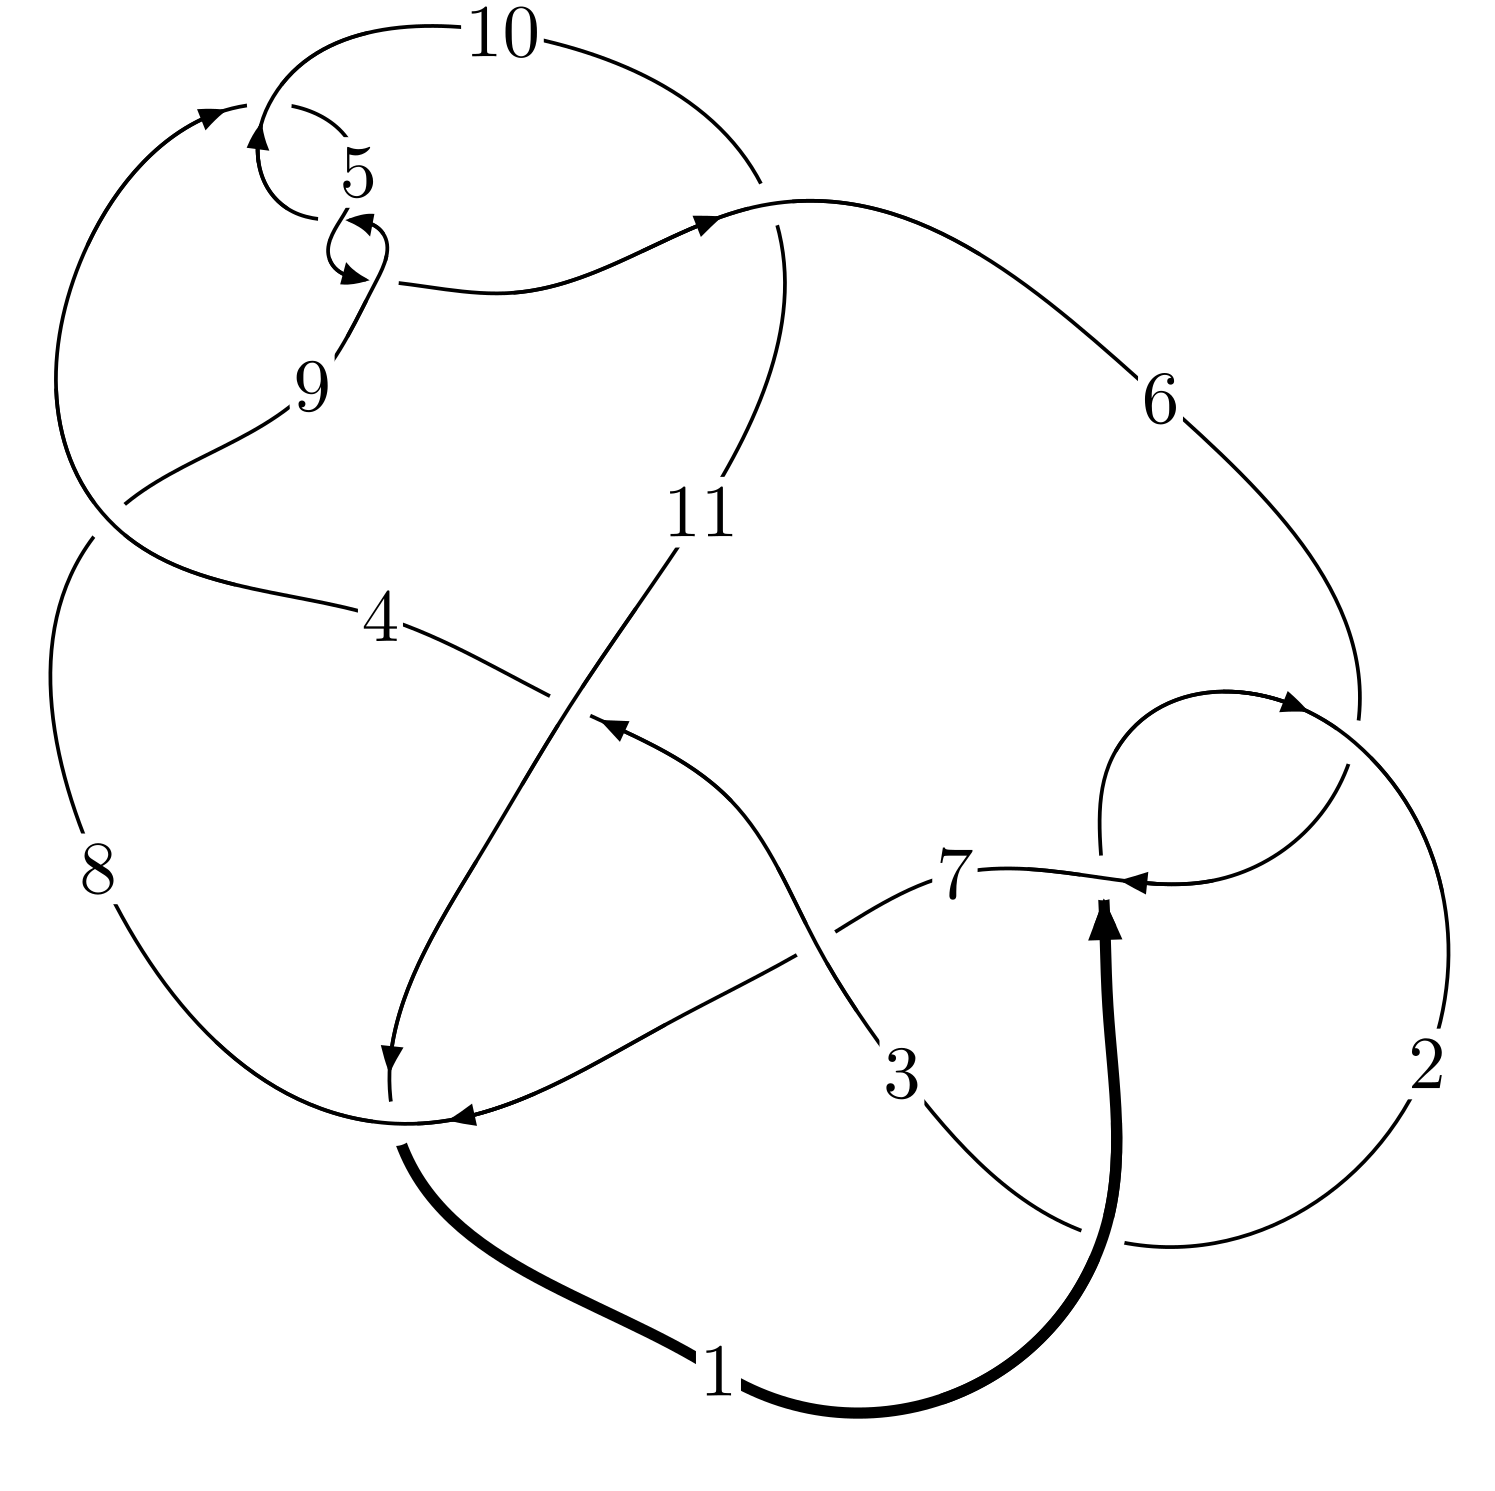
\includegraphics[width=112pt]{../../../GIT/diagram.site/Diagrams/png/432_11a_183.png}\\
\ \ \ A knot diagram\footnotemark}&
\allowdisplaybreaks
\textbf{Linearized knot diagam} \\
\cline{2-2}
 &
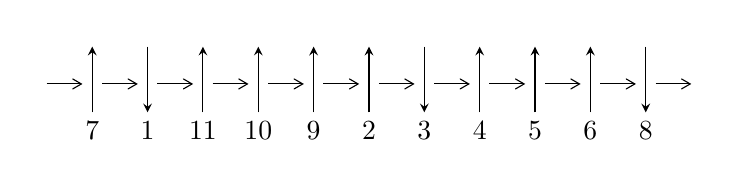
\begin{tikzpicture}[x=20pt, y=17pt]
	% nodes
	\node (C0) at (0, 0) {};
	\node (C1) at (1, 0) {};
	\node (C1U) at (1, +1) {};
	\node (C1D) at (1, -1) {7};

	\node (C2) at (2, 0) {};
	\node (C2U) at (2, +1) {};
	\node (C2D) at (2, -1) {1};

	\node (C3) at (3, 0) {};
	\node (C3U) at (3, +1) {};
	\node (C3D) at (3, -1) {11};

	\node (C4) at (4, 0) {};
	\node (C4U) at (4, +1) {};
	\node (C4D) at (4, -1) {10};

	\node (C5) at (5, 0) {};
	\node (C5U) at (5, +1) {};
	\node (C5D) at (5, -1) {9};

	\node (C6) at (6, 0) {};
	\node (C6U) at (6, +1) {};
	\node (C6D) at (6, -1) {2};

	\node (C7) at (7, 0) {};
	\node (C7U) at (7, +1) {};
	\node (C7D) at (7, -1) {3};

	\node (C8) at (8, 0) {};
	\node (C8U) at (8, +1) {};
	\node (C8D) at (8, -1) {4};

	\node (C9) at (9, 0) {};
	\node (C9U) at (9, +1) {};
	\node (C9D) at (9, -1) {5};

	\node (C10) at (10, 0) {};
	\node (C10U) at (10, +1) {};
	\node (C10D) at (10, -1) {6};

	\node (C11) at (11, 0) {};
	\node (C11U) at (11, +1) {};
	\node (C11D) at (11, -1) {8};
	\node (C12) at (12, 0) {};

	% arrows
	\draw[->,>={angle 60}]
	(C0) edge (C1) (C1) edge (C2) (C2) edge (C3) (C3) edge (C4) (C4) edge (C5) (C5) edge (C6) (C6) edge (C7) (C7) edge (C8) (C8) edge (C9) (C9) edge (C10) (C10) edge (C11) (C11) edge (C12) ;	\draw[->,>=stealth]
	(C1D) edge (C1U) (C2U) edge (C2D) (C3D) edge (C3U) (C4D) edge (C4U) (C5D) edge (C5U) (C6D) edge (C6U) (C7U) edge (C7D) (C8D) edge (C8U) (C9D) edge (C9U) (C10D) edge (C10U) (C11U) edge (C11D) ;
	\end{tikzpicture} \\
\hhline{~~} \\& 
\textbf{Solving Sequence} \\ \cline{2-2} 
 &
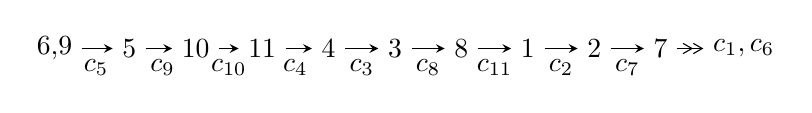
\begin{tikzpicture}[x=24pt, y=7pt]
	% node
	\node (A0) at (-1/8, 0) {6,9};
	\node (A1) at (1, 0) {5};
	\node (A2) at (2, 0) {10};
	\node (A3) at (3, 0) {11};
	\node (A4) at (4, 0) {4};
	\node (A5) at (5, 0) {3};
	\node (A6) at (6, 0) {8};
	\node (A7) at (7, 0) {1};
	\node (A8) at (8, 0) {2};
	\node (A9) at (9, 0) {7};
	\node (C1) at (1/2, -1) {$c_{5}$};
	\node (C2) at (3/2, -1) {$c_{9}$};
	\node (C3) at (5/2, -1) {$c_{10}$};
	\node (C4) at (7/2, -1) {$c_{4}$};
	\node (C5) at (9/2, -1) {$c_{3}$};
	\node (C6) at (11/2, -1) {$c_{8}$};
	\node (C7) at (13/2, -1) {$c_{11}$};
	\node (C8) at (15/2, -1) {$c_{2}$};
	\node (C9) at (17/2, -1) {$c_{7}$};
	\node (A10) at (41/4, 0) {$c_{1},c_{6}$};

	% edge
	\draw[->,>=stealth]	
	(A0) edge (A1) (A1) edge (A2) (A2) edge (A3) (A3) edge (A4) (A4) edge (A5) (A5) edge (A6) (A6) edge (A7) (A7) edge (A8) (A8) edge (A9) ;
	\draw[->>,>={angle 60}]	
	(A9) edge (A10);
\end{tikzpicture} \\ 

\end{tabular} \\

\footnotetext{
The image of knot diagram is generated by the software ``\textbf{Draw programme}" developed by Andrew Bartholomew(\url{http://www.layer8.co.uk/maths/draw/index.htm\#Running-draw}), where we modified some parts for our purpose(\url{https://github.com/CATsTAILs/LinksPainter}).
}\phantom \\ \newline 
\centering \textbf{Ideals for irreducible components\footnotemark of $X_{\text{par}}$} 
 
\begin{align*}
I^u_{1}&=\langle 
u^{57}+u^{56}+\cdots+u+1\rangle \\
\\
\end{align*}
\raggedright * 1 irreducible components of $\dim_{\mathbb{C}}=0$, with total 57 representations.\\
\footnotetext{All coefficients of polynomials are rational numbers. But the coefficients are sometimes approximated in decimal forms when there is not enough margin.}
\newpage
\renewcommand{\arraystretch}{1}
\centering \section*{I. $I^u_{1}= \langle u^{57}+u^{56}+\cdots+u+1 \rangle$}
\flushleft \textbf{(i) Arc colorings}\\
\begin{tabular}{m{7pt} m{180pt} m{7pt} m{180pt} }
\flushright $a_{6}=$&$\begin{pmatrix}1\\0\end{pmatrix}$ \\
\flushright $a_{9}=$&$\begin{pmatrix}0\\u\end{pmatrix}$ \\
\flushright $a_{5}=$&$\begin{pmatrix}1\\u^2\end{pmatrix}$ \\
\flushright $a_{10}=$&$\begin{pmatrix}u\\u^3+u\end{pmatrix}$ \\
\flushright $a_{11}=$&$\begin{pmatrix}u^3+2 u\\u^3+u\end{pmatrix}$ \\
\flushright $a_{4}=$&$\begin{pmatrix}u^2+1\\u^4+2 u^2\end{pmatrix}$ \\
\flushright $a_{3}=$&$\begin{pmatrix}- u^{10}-5 u^8-8 u^6-3 u^4+3 u^2+1\\- u^{10}-4 u^8-5 u^6+3 u^2\end{pmatrix}$ \\
\flushright $a_{8}=$&$\begin{pmatrix}- u^5-2 u^3- u\\- u^7-3 u^5-2 u^3+u\end{pmatrix}$ \\
\flushright $a_{1}=$&$\begin{pmatrix}u^{15}+6 u^{13}+14 u^{11}+14 u^9+2 u^7-6 u^5-2 u^3+2 u\\u^{17}+7 u^{15}+19 u^{13}+22 u^{11}+3 u^9-14 u^7-6 u^5+4 u^3+u\end{pmatrix}$ \\
\flushright $a_{2}=$&$\begin{pmatrix}u^{42}+17 u^{40}+\cdots+u^2+1\\u^{44}+18 u^{42}+\cdots-5 u^4+2 u^2\end{pmatrix}$ \\
\flushright $a_{7}=$&$\begin{pmatrix}- u^{27}-12 u^{25}+\cdots+2 u^5+5 u^3\\- u^{27}-11 u^{25}+\cdots+u^3+u\end{pmatrix}$\\ \flushright $a_{7}=$&$\begin{pmatrix}- u^{27}-12 u^{25}+\cdots+2 u^5+5 u^3\\- u^{27}-11 u^{25}+\cdots+u^3+u\end{pmatrix}$\\&\end{tabular}
\flushleft \textbf{(ii) Obstruction class $= -1$}\\~\\
\flushleft \textbf{(iii) Cusp Shapes $= 4 u^{56}+4 u^{55}+\cdots-4 u^2+6$}\\~\\
\newpage\renewcommand{\arraystretch}{1}
\flushleft \textbf{(iv) u-Polynomials at the component}\newline \\
\begin{tabular}{m{50pt}|m{274pt}}
Crossings & \hspace{64pt}u-Polynomials at each crossing \\
\hline $$\begin{aligned}c_{1},c_{6}\end{aligned}$$&$\begin{aligned}
&u^{57}+u^{56}+\cdots- u-1
\end{aligned}$\\
\hline $$\begin{aligned}c_{2}\end{aligned}$$&$\begin{aligned}
&u^{57}+27 u^{56}+\cdots+u-1
\end{aligned}$\\
\hline $$\begin{aligned}c_{3}\end{aligned}$$&$\begin{aligned}
&u^{57}+7 u^{56}+\cdots+49 u+5
\end{aligned}$\\
\hline $$\begin{aligned}c_{4},c_{5},c_{9}\end{aligned}$$&$\begin{aligned}
&u^{57}- u^{56}+\cdots+u-1
\end{aligned}$\\
\hline $$\begin{aligned}c_{7}\end{aligned}$$&$\begin{aligned}
&u^{57}- u^{56}+\cdots+231 u-53
\end{aligned}$\\
\hline $$\begin{aligned}c_{8},c_{10}\end{aligned}$$&$\begin{aligned}
&u^{57}+u^{56}+\cdots-29 u-17
\end{aligned}$\\
\hline $$\begin{aligned}c_{11}\end{aligned}$$&$\begin{aligned}
&u^{57}+5 u^{56}+\cdots-264 u-112
\end{aligned}$\\
\hline
\end{tabular}\\~\\
\newpage\renewcommand{\arraystretch}{1}
\flushleft \textbf{(v) Riley Polynomials at the component}\newline \\
\begin{tabular}{m{50pt}|m{274pt}}
Crossings & \hspace{64pt}Riley Polynomials at each crossing \\
\hline $$\begin{aligned}c_{1},c_{6}\end{aligned}$$&$\begin{aligned}
&y^{57}+27 y^{56}+\cdots+y-1
\end{aligned}$\\
\hline $$\begin{aligned}c_{2}\end{aligned}$$&$\begin{aligned}
&y^{57}+7 y^{56}+\cdots-3 y-1
\end{aligned}$\\
\hline $$\begin{aligned}c_{3}\end{aligned}$$&$\begin{aligned}
&y^{57}+3 y^{56}+\cdots-519 y-25
\end{aligned}$\\
\hline $$\begin{aligned}c_{4},c_{5},c_{9}\end{aligned}$$&$\begin{aligned}
&y^{57}+47 y^{56}+\cdots+y-1
\end{aligned}$\\
\hline $$\begin{aligned}c_{7}\end{aligned}$$&$\begin{aligned}
&y^{57}-13 y^{56}+\cdots+82617 y-2809
\end{aligned}$\\
\hline $$\begin{aligned}c_{8},c_{10}\end{aligned}$$&$\begin{aligned}
&y^{57}-37 y^{56}+\cdots-1267 y-289
\end{aligned}$\\
\hline $$\begin{aligned}c_{11}\end{aligned}$$&$\begin{aligned}
&y^{57}+15 y^{56}+\cdots-381664 y-12544
\end{aligned}$\\
\hline
\end{tabular}\\~\\
\newpage\flushleft \textbf{(vi) Complex Volumes and Cusp Shapes}
$$\begin{array}{c|c|c}  
\text{Solutions to }I^u_{1}& \I (\text{vol} + \sqrt{-1}CS) & \text{Cusp shape}\\
 \hline 
\begin{aligned}
u &= -0.277649 + 1.138010 I\end{aligned}
 & -2.98923 - 1.15216 I & \phantom{-0.000000 } 0 \\ \hline\begin{aligned}
u &= -0.277649 - 1.138010 I\end{aligned}
 & -2.98923 + 1.15216 I & \phantom{-0.000000 } 0 \\ \hline\begin{aligned}
u &= -0.343977 + 1.120270 I\end{aligned}
 & -0.58525 + 6.08343 I & \phantom{-0.000000 } 0 \\ \hline\begin{aligned}
u &= -0.343977 - 1.120270 I\end{aligned}
 & -0.58525 - 6.08343 I & \phantom{-0.000000 } 0 \\ \hline\begin{aligned}
u &= -0.804549 + 0.125513 I\end{aligned}
 & \phantom{-}2.43881 - 10.27360 I & \phantom{-}7.12723 + 7.98252 I \\ \hline\begin{aligned}
u &= -0.804549 - 0.125513 I\end{aligned}
 & \phantom{-}2.43881 + 10.27360 I & \phantom{-}7.12723 - 7.98252 I \\ \hline\begin{aligned}
u &= \phantom{-}0.337618 + 1.140540 I\end{aligned}
 & \phantom{-}1.53395 - 1.08977 I & \phantom{-0.000000 } 0 \\ \hline\begin{aligned}
u &= \phantom{-}0.337618 - 1.140540 I\end{aligned}
 & \phantom{-}1.53395 + 1.08977 I & \phantom{-0.000000 } 0 \\ \hline\begin{aligned}
u &= \phantom{-}0.799720 + 0.113827 I\end{aligned}
 & \phantom{-}4.65256 + 5.23405 I & \phantom{-}10.45155 - 4.02810 I \\ \hline\begin{aligned}
u &= \phantom{-}0.799720 - 0.113827 I\end{aligned}
 & \phantom{-}4.65256 - 5.23405 I & \phantom{-}10.45155 + 4.02810 I \\ \hline\begin{aligned}
u &= \phantom{-}0.797777 + 0.076863 I\end{aligned}
 & \phantom{-}5.78308 + 2.96634 I & \phantom{-}12.01643 - 3.84738 I \\ \hline\begin{aligned}
u &= \phantom{-}0.797777 - 0.076863 I\end{aligned}
 & \phantom{-}5.78308 - 2.96634 I & \phantom{-}12.01643 + 3.84738 I \\ \hline\begin{aligned}
u &= -0.798784 + 0.053217 I\end{aligned}
 & \phantom{-}4.63483 + 1.87363 I & \phantom{-}10.12440 - 2.27509 I \\ \hline\begin{aligned}
u &= -0.798784 - 0.053217 I\end{aligned}
 & \phantom{-}4.63483 - 1.87363 I & \phantom{-}10.12440 + 2.27509 I \\ \hline\begin{aligned}
u &= -0.771308 + 0.122509 I\end{aligned}
 & \phantom{-}0.04467 - 2.73028 I & \phantom{-}4.01382 + 2.71873 I \\ \hline\begin{aligned}
u &= -0.771308 - 0.122509 I\end{aligned}
 & \phantom{-}0.04467 + 2.73028 I & \phantom{-}4.01382 - 2.71873 I \\ \hline\begin{aligned}
u &= \phantom{-}0.342759 + 1.189140 I\end{aligned}
 & \phantom{-}2.38357 + 1.16168 I & \phantom{-0.000000 } 0 \\ \hline\begin{aligned}
u &= \phantom{-}0.342759 - 1.189140 I\end{aligned}
 & \phantom{-}2.38357 - 1.16168 I & \phantom{-0.000000 } 0 \\ \hline\begin{aligned}
u &= -0.348811 + 1.212550 I\end{aligned}
 & \phantom{-}1.07430 - 6.01691 I & \phantom{-0.000000 } 0 \\ \hline\begin{aligned}
u &= -0.348811 - 1.212550 I\end{aligned}
 & \phantom{-}1.07430 + 6.01691 I & \phantom{-0.000000 } 0 \\ \hline\begin{aligned}
u &= -0.052037 + 1.291330 I\end{aligned}
 & -3.68835 - 1.96306 I & \phantom{-0.000000 } 0 \\ \hline\begin{aligned}
u &= -0.052037 - 1.291330 I\end{aligned}
 & -3.68835 + 1.96306 I & \phantom{-0.000000 } 0 \\ \hline\begin{aligned}
u &= -0.266975 + 1.304600 I\end{aligned}
 & -2.86692 - 3.28224 I & \phantom{-0.000000 } 0 \\ \hline\begin{aligned}
u &= -0.266975 - 1.304600 I\end{aligned}
 & -2.86692 + 3.28224 I & \phantom{-0.000000 } 0 \\ \hline\begin{aligned}
u &= \phantom{-}0.236806 + 1.324490 I\end{aligned}
 & -5.56866 - 0.84775 I & \phantom{-0.000000 } 0 \\ \hline\begin{aligned}
u &= \phantom{-}0.236806 - 1.324490 I\end{aligned}
 & -5.56866 + 0.84775 I & \phantom{-0.000000 } 0 \\ \hline\begin{aligned}
u &= -0.346838 + 1.301460 I\end{aligned}
 & \phantom{-}0.40457 - 2.25231 I & \phantom{-0.000000 } 0 \\ \hline\begin{aligned}
u &= -0.346838 - 1.301460 I\end{aligned}
 & \phantom{-}0.40457 + 2.25231 I & \phantom{-0.000000 } 0 \\ \hline\begin{aligned}
u &= \phantom{-}0.634619 + 0.140548 I\end{aligned}
 & -1.62790 + 3.37240 I & \phantom{-}3.27495 - 5.30685 I \\ \hline\begin{aligned}
u &= \phantom{-}0.634619 - 0.140548 I\end{aligned}
 & -1.62790 - 3.37240 I & \phantom{-}3.27495 + 5.30685 I\\
 \hline 
 \end{array}$$\newpage$$\begin{array}{c|c|c}  
\text{Solutions to }I^u_{1}& \I (\text{vol} + \sqrt{-1}CS) & \text{Cusp shape}\\
 \hline 
\begin{aligned}
u &= -0.638377\phantom{ +0.000000I}\end{aligned}
 & \phantom{-}1.27831\phantom{ +0.000000I} & \phantom{-}8.28660\phantom{ +0.000000I} \\ \hline\begin{aligned}
u &= \phantom{-}0.346920 + 1.317510 I\end{aligned}
 & \phantom{-}1.41577 + 7.09232 I & \phantom{-0.000000 } 0 \\ \hline\begin{aligned}
u &= \phantom{-}0.346920 - 1.317510 I\end{aligned}
 & \phantom{-}1.41577 - 7.09232 I & \phantom{-0.000000 } 0 \\ \hline\begin{aligned}
u &= \phantom{-}0.277893 + 1.335410 I\end{aligned}
 & -6.25104 + 6.75305 I & \phantom{-0.000000 } 0 \\ \hline\begin{aligned}
u &= \phantom{-}0.277893 - 1.335410 I\end{aligned}
 & -6.25104 - 6.75305 I & \phantom{-0.000000 } 0 \\ \hline\begin{aligned}
u &= \phantom{-}0.337361 + 0.533102 I\end{aligned}
 & -1.72047 + 6.62089 I & \phantom{-}2.54306 - 8.39817 I \\ \hline\begin{aligned}
u &= \phantom{-}0.337361 - 0.533102 I\end{aligned}
 & -1.72047 - 6.62089 I & \phantom{-}2.54306 + 8.39817 I \\ \hline\begin{aligned}
u &= -0.058345 + 1.369800 I\end{aligned}
 & -5.26507 - 3.02226 I & \phantom{-0.000000 } 0 \\ \hline\begin{aligned}
u &= -0.058345 - 1.369800 I\end{aligned}
 & -5.26507 + 3.02226 I & \phantom{-0.000000 } 0 \\ \hline\begin{aligned}
u &= -0.331323 + 1.341910 I\end{aligned}
 & -4.56299 - 6.72032 I & \phantom{-0.000000 } 0 \\ \hline\begin{aligned}
u &= -0.331323 - 1.341910 I\end{aligned}
 & -4.56299 + 6.72032 I & \phantom{-0.000000 } 0 \\ \hline\begin{aligned}
u &= \phantom{-}0.032432 + 1.383040 I\end{aligned}
 & -9.34182 + 0.07828 I & \phantom{-0.000000 } 0 \\ \hline\begin{aligned}
u &= \phantom{-}0.032432 - 1.383040 I\end{aligned}
 & -9.34182 - 0.07828 I & \phantom{-0.000000 } 0 \\ \hline\begin{aligned}
u &= \phantom{-}0.346087 + 1.339690 I\end{aligned}
 & \phantom{-}0.08340 + 9.36804 I & \phantom{-0.000000 } 0 \\ \hline\begin{aligned}
u &= \phantom{-}0.346087 - 1.339690 I\end{aligned}
 & \phantom{-}0.08340 - 9.36804 I & \phantom{-0.000000 } 0 \\ \hline\begin{aligned}
u &= \phantom{-}0.063733 + 1.386370 I\end{aligned}
 & -7.68595 + 7.77424 I & \phantom{-0.000000 } 0 \\ \hline\begin{aligned}
u &= \phantom{-}0.063733 - 1.386370 I\end{aligned}
 & -7.68595 - 7.77424 I & \phantom{-0.000000 } 0 \\ \hline\begin{aligned}
u &= -0.347692 + 1.346470 I\end{aligned}
 & -2.1926 - 14.4304 I & \phantom{-0.000000 } 0 \\ \hline\begin{aligned}
u &= -0.347692 - 1.346470 I\end{aligned}
 & -2.1926 + 14.4304 I & \phantom{-0.000000 } 0 \\ \hline\begin{aligned}
u &= \phantom{-}0.192189 + 0.576599 I\end{aligned}
 & -3.37572 - 0.51768 I & -1.48190 - 0.98551 I \\ \hline\begin{aligned}
u &= \phantom{-}0.192189 - 0.576599 I\end{aligned}
 & -3.37572 + 0.51768 I & -1.48190 + 0.98551 I \\ \hline\begin{aligned}
u &= -0.310416 + 0.472368 I\end{aligned}
 & \phantom{-}0.42908 - 1.95168 I & \phantom{-}6.05217 + 4.83311 I \\ \hline\begin{aligned}
u &= -0.310416 - 0.472368 I\end{aligned}
 & \phantom{-}0.42908 + 1.95168 I & \phantom{-}6.05217 - 4.83311 I \\ \hline\begin{aligned}
u &= \phantom{-}0.499130 + 0.251121 I\end{aligned}
 & -0.85109 - 3.57978 I & \phantom{-}5.03586 + 1.38706 I \\ \hline\begin{aligned}
u &= \phantom{-}0.499130 - 0.251121 I\end{aligned}
 & -0.85109 + 3.57978 I & \phantom{-}5.03586 - 1.38706 I \\ \hline\begin{aligned}
u &= -0.367153 + 0.287513 I\end{aligned}
 & \phantom{-}0.979056 - 0.679070 I & \phantom{-}8.79507 + 4.86357 I \\ \hline\begin{aligned}
u &= -0.367153 - 0.287513 I\end{aligned}
 & \phantom{-}0.979056 + 0.679070 I & \phantom{-}8.79507 - 4.86357 I\\
 \hline 
 \end{array}$$\newpage
\newpage\renewcommand{\arraystretch}{1}
\centering \section*{ II. u-Polynomials}
\begin{tabular}{m{50pt}|m{274pt}}
Crossings & \hspace{64pt}u-Polynomials at each crossing \\
\hline $$\begin{aligned}c_{1},c_{6}\end{aligned}$$&$\begin{aligned}
&u^{57}+u^{56}+\cdots- u-1
\end{aligned}$\\
\hline $$\begin{aligned}c_{2}\end{aligned}$$&$\begin{aligned}
&u^{57}+27 u^{56}+\cdots+u-1
\end{aligned}$\\
\hline $$\begin{aligned}c_{3}\end{aligned}$$&$\begin{aligned}
&u^{57}+7 u^{56}+\cdots+49 u+5
\end{aligned}$\\
\hline $$\begin{aligned}c_{4},c_{5},c_{9}\end{aligned}$$&$\begin{aligned}
&u^{57}- u^{56}+\cdots+u-1
\end{aligned}$\\
\hline $$\begin{aligned}c_{7}\end{aligned}$$&$\begin{aligned}
&u^{57}- u^{56}+\cdots+231 u-53
\end{aligned}$\\
\hline $$\begin{aligned}c_{8},c_{10}\end{aligned}$$&$\begin{aligned}
&u^{57}+u^{56}+\cdots-29 u-17
\end{aligned}$\\
\hline $$\begin{aligned}c_{11}\end{aligned}$$&$\begin{aligned}
&u^{57}+5 u^{56}+\cdots-264 u-112
\end{aligned}$\\
\hline
\end{tabular}\newpage\renewcommand{\arraystretch}{1}
\centering \section*{ III. Riley Polynomials}
\begin{tabular}{m{50pt}|m{274pt}}
Crossings & \hspace{64pt}Riley Polynomials at each crossing \\
\hline $$\begin{aligned}c_{1},c_{6}\end{aligned}$$&$\begin{aligned}
&y^{57}+27 y^{56}+\cdots+y-1
\end{aligned}$\\
\hline $$\begin{aligned}c_{2}\end{aligned}$$&$\begin{aligned}
&y^{57}+7 y^{56}+\cdots-3 y-1
\end{aligned}$\\
\hline $$\begin{aligned}c_{3}\end{aligned}$$&$\begin{aligned}
&y^{57}+3 y^{56}+\cdots-519 y-25
\end{aligned}$\\
\hline $$\begin{aligned}c_{4},c_{5},c_{9}\end{aligned}$$&$\begin{aligned}
&y^{57}+47 y^{56}+\cdots+y-1
\end{aligned}$\\
\hline $$\begin{aligned}c_{7}\end{aligned}$$&$\begin{aligned}
&y^{57}-13 y^{56}+\cdots+82617 y-2809
\end{aligned}$\\
\hline $$\begin{aligned}c_{8},c_{10}\end{aligned}$$&$\begin{aligned}
&y^{57}-37 y^{56}+\cdots-1267 y-289
\end{aligned}$\\
\hline $$\begin{aligned}c_{11}\end{aligned}$$&$\begin{aligned}
&y^{57}+15 y^{56}+\cdots-381664 y-12544
\end{aligned}$\\
\hline
\end{tabular}
\vskip 2pc
\end{document}